\section{Proposed Approach: \\ \textit{Reverse-Engineering Language Product Lines}}
\label{sec:approach}

In this section, we present our reverse engineering technique to support the construction of bottom-up language product lines. As shown in Fig. \ref{fig:reverse-engineering}, the proposed technique is composed of three steps. During the first step, we automatically recover a language modular design for the language product line. Such a modular design is composed of a set of language modules and a set of dependencies among them. During the second step, language modules' dependencies are used to synthesize a variability model that can be used, during the third step, to configure concrete DSL variants. Finally, during the forth step the DSL variant is assembled by composing the involved language modules. 

\begin{figure*}
\centering
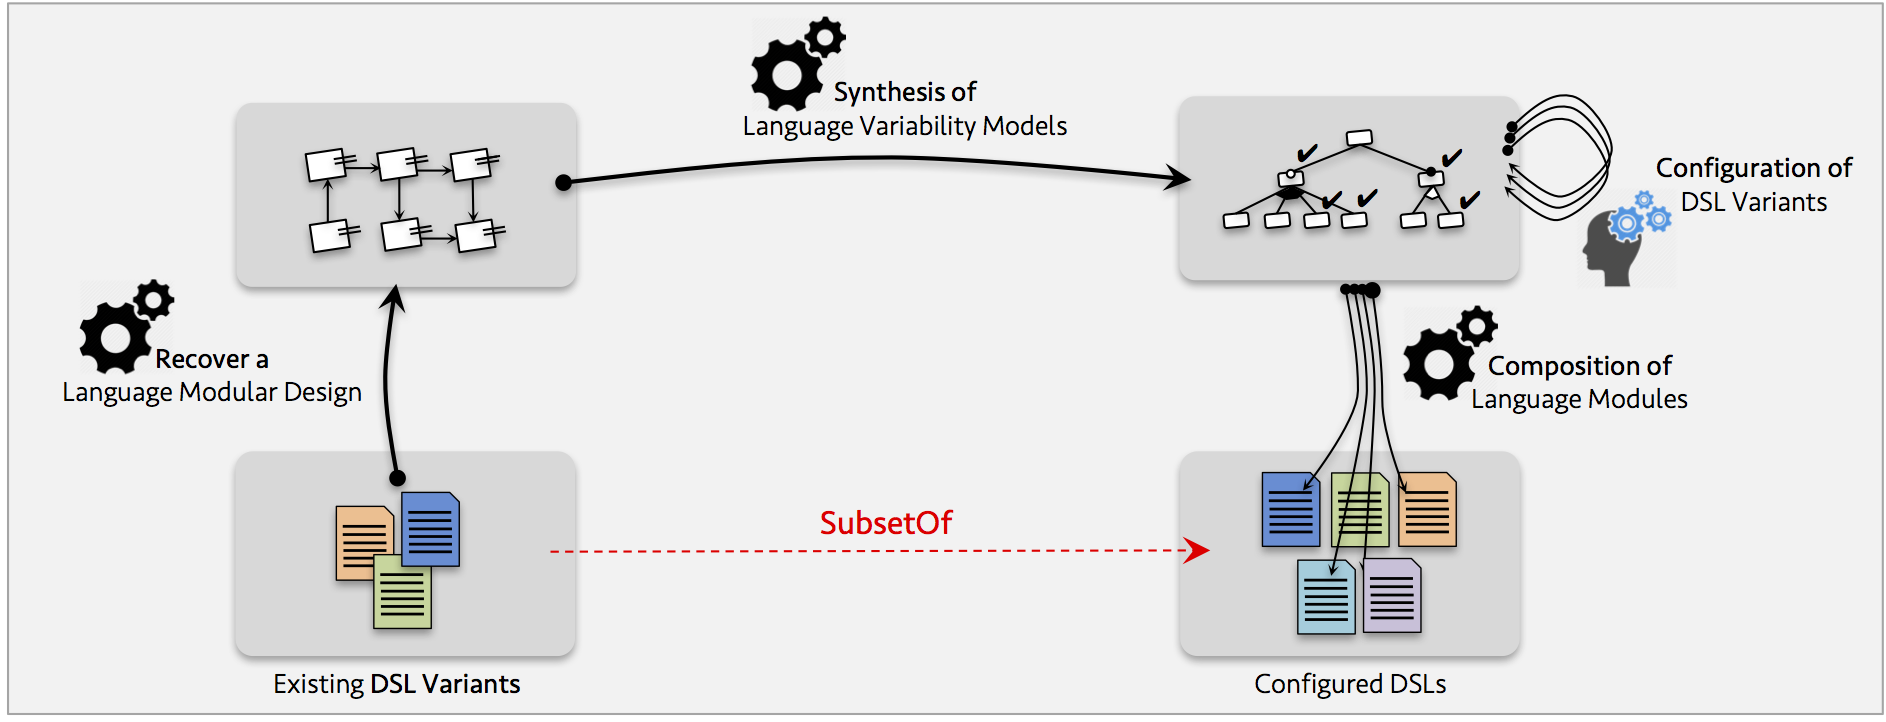
\includegraphics[width=1\linewidth]{images/reverse-engineering-overview.png}
\caption{Reverse engineering language product lines: approach overview}
\label{fig:reverse-engineering}
\end{figure*}

\subsection{Recovering a Language Modular Design}
\label{sec:reverseengineeringmodules}

Let us start the description of our reverse engineering technique by explaining the way in which we identify the set of language modules and dependencies that constitute the language modular design of the product line. The details of this recovering process are explained below as well as the way in which language modules are specified to guarantee their composability. 

\subsubsection{Language Modules. \textbf{How to identify them?}}

To identify the language modules of a language product line, we define some comparison operators that facilitate the identification of language constructs replicated in the DSL variants. These operators take into account both syntax and semantics of language constructs. Then, we extract replicated constructs into interdependent language modules whose dependencies are expressed through interfaces guaranteeing that those language modules can be later assembled among them. Such a strategy to extract reusable language modules is based on four principles explained in the following:

\vspace{1mm}
\emph{\textbf{Principle 1:} DSL specifications are comparable. So, replicated language constructs can be automatically detected.} To detect replicated language constructs in a given set of DSL variants, we need to define some criteria to compare the DSL specifications to decide when a language construct is equal to another. For the technological space discussed in this article, a language construct is defined in terms of a metaclass and a set of domain specific actions. 

\vspace{1mm}
\emph{Comparison of metaclasses.} To compare metaclasses, we need to take into account that a metaclass is specified by a name, a set of attributes, and a set of references to other metaclasses. Two metaclasses are considered as equal if all those elements match. Formally, comparison of metaclasses is formalized by the operator $\doteqdot$.

\begin{equation}
  \doteqdot~: MC \times MC \rightarrow bool
\end{equation}
\begin{equation}
\begin{split}
  MC_{A} &\doteqdot MC_{B} = true \implies \\
   & MC_{A}.name = MC_{B}.name ~ \wedge \\
   & \forall a_1 \in MC_{A}.attr \mid (\exists a_2 \in MC_{B}.attr \mid a_1 = a_2) ~ \wedge \\
   & \forall r_1 \in MC_{A}.refs \mid (\exists r_2 \in MC_{B}.refs \mid r_1 = r_2) ~ \wedge \\
   & |MC_{A}.attr| = |MC_{B}.attr| ~ \wedge \\
   & |MC_{A}.refs| = |MC_{B}.refs|
  \end{split}
\end{equation}

\emph{Comparison of domain-specific actions.} To compare domain specific actions, we need to consider that --similarly to methods in Java-- domain specific actions have a signature that specifies its contract (i.e., return type, visibility, parameters, name, and so on), and a body where the behavior is implemented. Two domain specific actions are equal if their signatures and bodies are equivalent.

Whereas comparison of signatures can be performed by syntactic comparison of the signature elements, comparison of bodies can be arbitrary difficult. If we try to compare the behavior of the domain-specific actions, then we will have to address the semantic equivalence problem, which is known to be undecidable \cite{Lucanu:2013}. To address this issue, we conceive bodies comparison in terms of its abstract syntax tree as proposed by Biegel et al. \cite{Biegel:2010}. In other words, to compare two bodies, we first parse them to extract their abstract syntax tree, and then we compare those trees. Formally, comparison of domain-specific actions (DSAs) is specified by the operator $\fallingdotseq$.  

\begin{equation}
  \fallingdotseq~: DSA \times DSA \rightarrow bool
\end{equation}
\begin{equation}
\begin{split}
  DSA_{A} & \fallingdotseq DSA_{B} = true \implies \\
   & DSA_{A}.name = DSA_{B}.name ~ \wedge \\
   & DSA_{A}.returnType = DSA_{B}.returnType ~ \wedge \\
   & DSA_{A}.visibility = DSA_{B}.visibility ~ \wedge \\
   & \forall p_1 \in DSA_{A}.params \mid \\
   & (\exists p_2 \in DSA_{B}.params \mid p_1 = p_2)  ~ \wedge \\
   & |DSA_{A}.params| = |DSA_{B}.params|  ~ \wedge \\
   & DSA_{A}.AST = DSA_{B}.AST
 \end{split}
\end{equation}

Note that these comparison operators are structural for both syntax and semantics of language constructs. They result useful when the DSL variants were built-up by using practices such as clone-and-clone. To enhance the scope of the approach, other comparison operators that take into accoung not only the structure of the constructs but their runtime behavior can be introduced. 

\vspace{2mm}
\emph{\textbf{Principle 2:} Replicated constructs can be viewed as sets' intersections, which is useful to factorization.} A DSL specification can be seen as a set of metaclasses and a set of domain specific actions. In doing so, replicated constructs correspond to intersections among those sets. Those intersection elements can be specified once and reused in several DSL variants \cite[p. 60-61]{Voelter:2013b}. Hence, we can factorize replication constructs by breaking down the intersections existing among DSL specifications.

\begin{figure*}[h!]
	\centering
	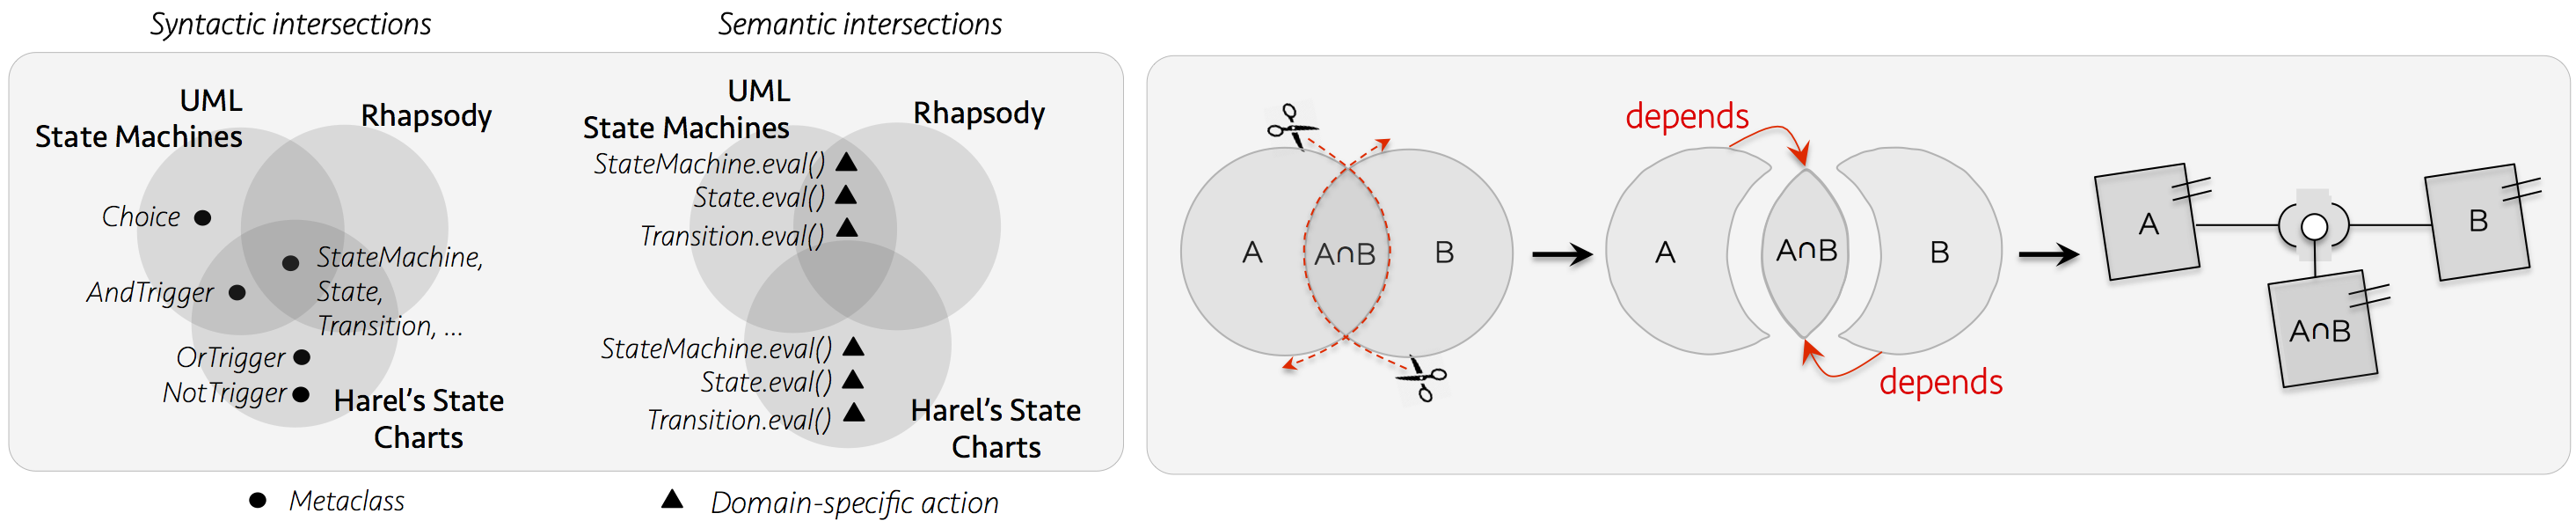
\includegraphics[width=1\linewidth]{images/principle2.png}
	\caption{Factorizing replicated language constructs from DSL variants}
	\label{fig:shape}
\end{figure*}

Fig. \ref{fig:shape} illustrates this observation through the running example introduced in Section \ref{sec:problemstatement}. At the left of the figure, we show two Venn diagrams to represent both syntax and semantic intersections. The Venn diagram corresponding to the abstract syntax shows that the classical constructs for state machines such as StateMachine, State, and Transition are in the intersection of the three given DSL variants i.e., UML state machines, Rhapsody, and Harel's state machines. In turn, there are certain particularities for each DSL. For example, the concept AndTrigger is owned by UML and Harel state machines but not for Rhapsody. Concepts such as OrTrigger and NotTrigger are only provided by Harel state machines since the concept of Choice is exclusive of UML state machines.

For the case of semantic variability, the 3-sets intersection is empty. It means that there is not a common semantic for the three DSL variants. Rather, UML state machines and Rhapsody share the domain specific actions corresponding to the constructs of State Machine, State, and Transition. In turn, the implementation of Harel state machines is different. 

This way to conceive DSL specifications is useful to factorize replicated language constructs as illustrated at the right of Fig. \ref{fig:shape}. Each different intersection is separated in a separate subset that, as we will explain later, is encapsulated in a language module. 



%\vspace{2mm}
%\textit{\textbf{Principle 3:} Breaking down overlapping is useful to factorize specification clones.} According to principle 2, overlapping between two DSLs implies the existence of repeated metaclasses and/or domain specific actions i.e., specification clones. Those repeated elements can be specified once and reused in the two DSLs \cite[p. 60-61]{Voelter:2013b}. Hence, we can factorize specification clones by breaking down the overlapping existing among DSL specifications as illustrated in Figure \ref{fig:cutting}; 

%\begin{figure}
%\centering
%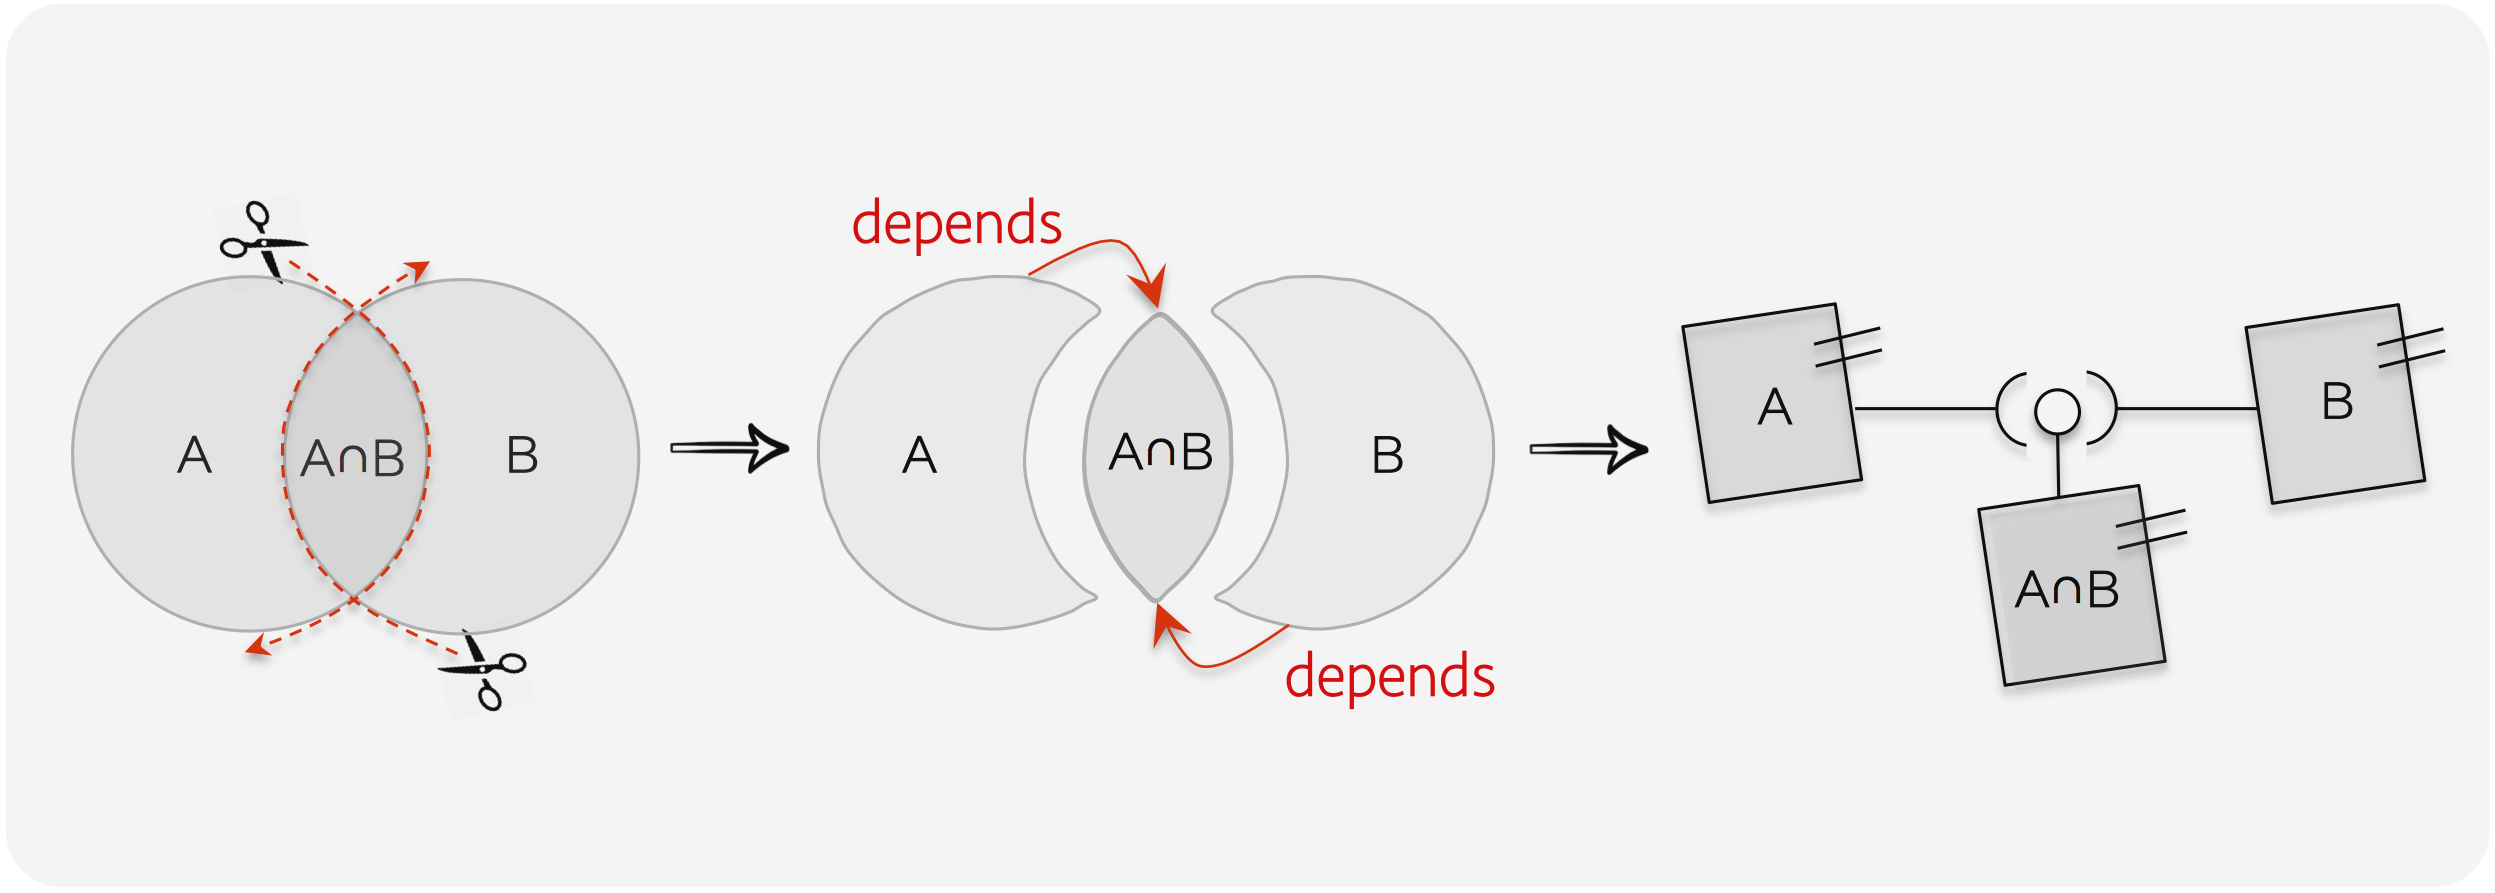
\includegraphics[width=0.97\linewidth]{images/fig-breaking-overlapping.png}
%\caption{Breaking down overlapping to obtain language modules}
%\label{fig:cutting}
%\end{figure}

\vspace{2mm}
\textit{\textbf{Principle 3:} Abstract syntax first, semantics afterwards.} The abstract syntax is the backbone of the DSL specification; it specifies its structure in terms of metaclasses and relationships among them whereas the domain-specific actions add executability to the metaclasses. Hence, the process of breaking down intersections should be performed for the abstract syntax first, thus identifying the way in which metaclasses should be grouped into the different language modules. Afterwards, we can do the proper for the semantics. In doing so, we need to take into consideration the phenomenon of semantic variability. That is, two replicated metaclasses might have different domain-specific actions. That occurs when two DSLs share some syntax specification but differ in their semantics.

\vspace{2mm}
\textit{\textbf{Principle 4:} Breaking down a metamodel is a graph partitioning problem.} A metamodel can be seen as a directed graph $G=<V,A>$ where:

\begin{itemize}
\item \textbf{V}: is the set of vertices each of which represents a metaclass.
\item \textbf{A}: is the set of arcs each of which represents a relationship between two metaclasses i.e., references, containments, and inheritances.
\end{itemize}

This observation is useful for breaking down metamodels, which can be viewed as a graph partitioning problem where the result is a finite set of subgraphs. Each subgraph represents the metamodel of a reusable language module.

\vspace{2mm}
\textbf{\textit{The principles in action.}} Fig. \ref{fig:breakingdown} shows the way in which we recover a language modular design through the principles explained above. It is composed of two steps: unification and breaking down.

\begin{figure*}
\centering
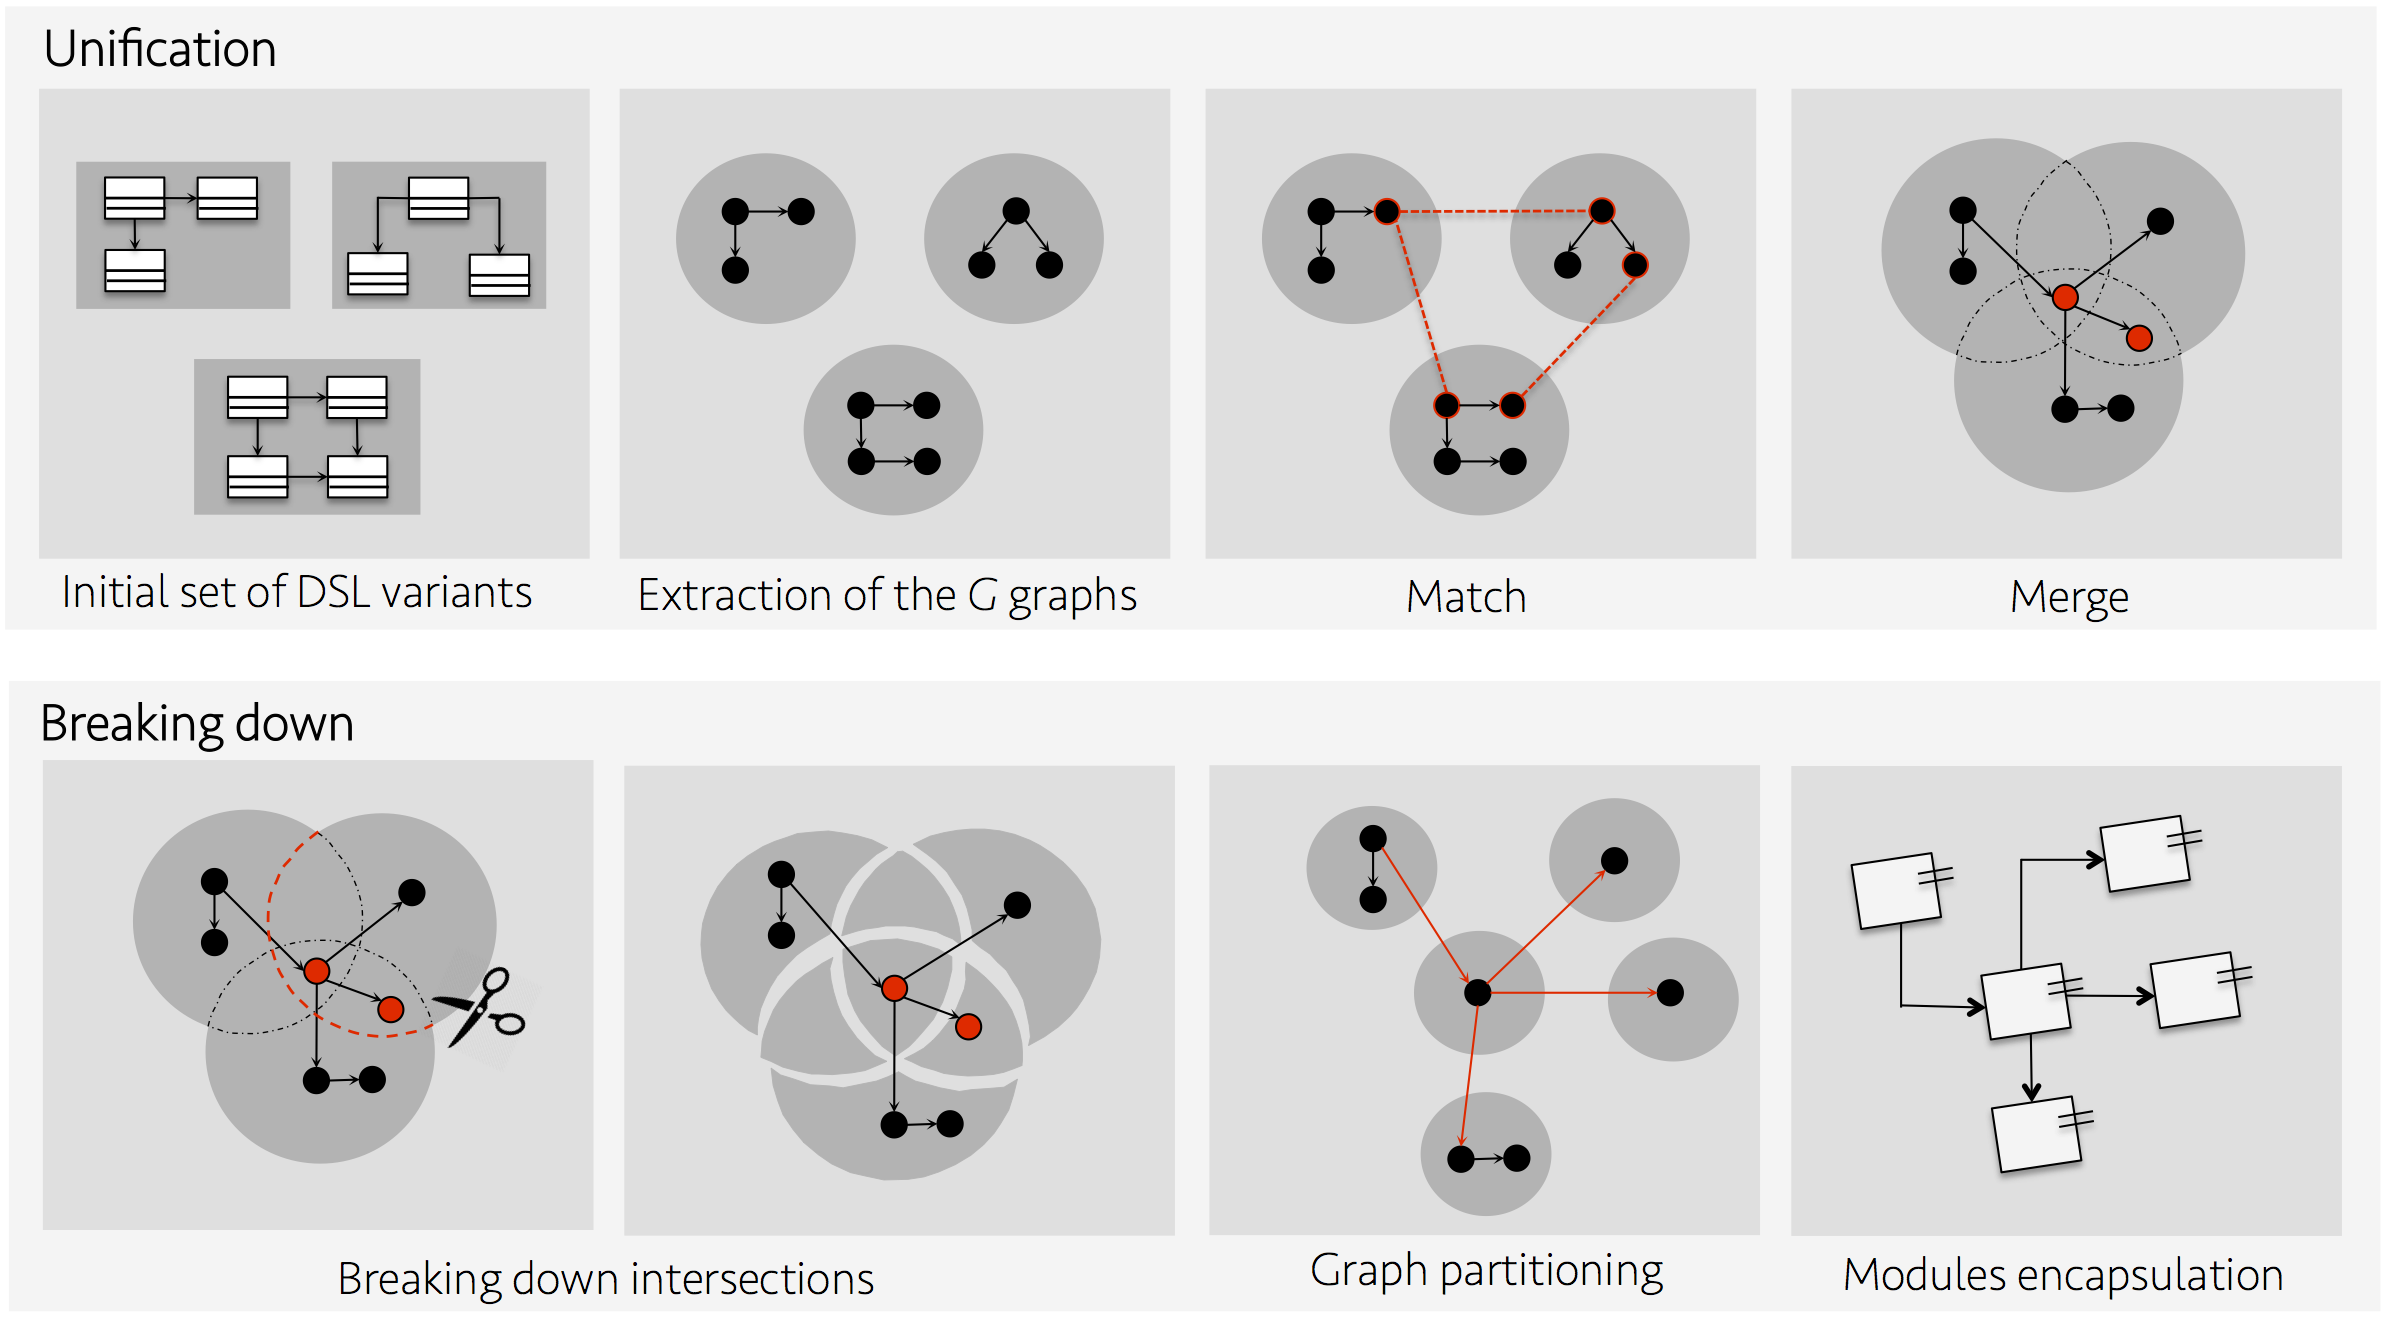
\includegraphics[width=1\linewidth]{images/fig-reverse-engineering-detailed.png}
\caption{Unifying and breaking down for recovering a language modular design}
\label{fig:breakingdown}
\end{figure*}

\vspace{2mm}
\textit{Unification: \textbf{match} and \textbf{merge}.} The objective of this step is to unify all the DSL variants in a unique specification. To this end, we first produce a graph $G$ for the metamodel of each DSL variant according to the principle 4. Second, we use the comparison operators defined in the principle 1 to match the vertices representing the metaclasses repeated in two or more DSL variants. Third, we create the syntactic intersections defined in principle 2 by merging the matched vertices. In doing so, we remove replicated metaclasses. After this process, we have a unified graph (which is not necessarily a connected graph) including all the metaclasses provided in the DSL variants. 

To identify semantic intersections, we check whether the domain specific actions of the matched metaclasses are equal. If so, they can be considered as semantic replications, and they are also merged. If not all the domain specific actions associated to the matched metaclasses are equal, different clusters of domain specific actions are created, thus establishing semantic variation points.

\vspace{2mm}
\textit{Breaking down: \textbf{cut} and \textbf{encapsulate}.} Once intersections among the DSL variants have been identified, we factorize the replicated language constructs. To this end, we break down the unified graph using a graph partitioning algorithm. Our algorithm returns a set of clusters of vertices: one cluster for each intersection of the Venn diagram. Arcs defined between vertices in different clusters can be considered as cross-cutting dependencies between clusters. Finally, we encapsulate each vertex cluster in the form of a language module. 

\subsubsection{Language Modules. \textbf{How to specify them?}}

We have explained the way in which we recover a language modular design by identifying clusters of language constructs and dependencies among them. However, it is unclear how to specify those clusters in concrete implementation artifacts that can be later composed. To answer deal with this issue, we propose to specify a language module in terms of (1) a metamodel containing the metaclasses corresponding to each construct cluster; and (2) a set of domain specific actions implementing the semantics of their metaclasses (see Fig. \ref{fig:modulespec}). If there is semantic variability, then a language module can have several clusters of domain specific actions. The dependencies among language modules are materialized through required and provided interfaces. 

\begin{figure}[h!]
\centering
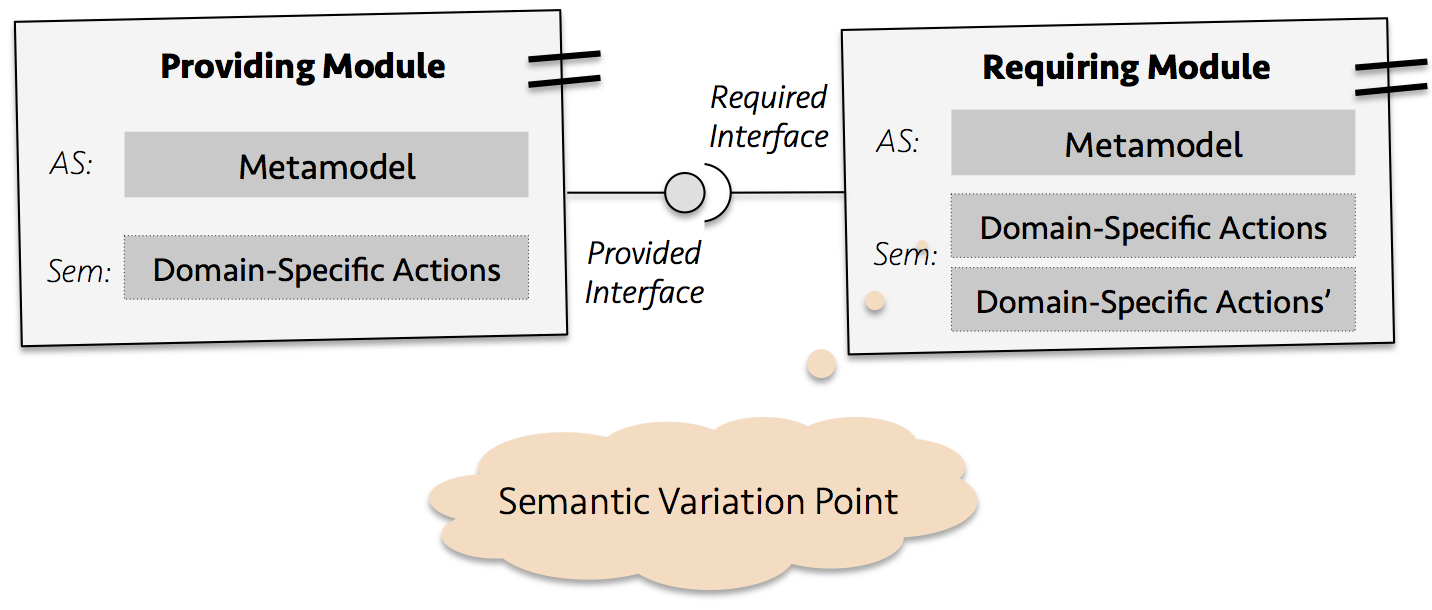
\includegraphics[width=1\linewidth]{images/language-modules-specification.png}
\caption{Specification of language modules}
\label{fig:modulespec}
\end{figure}



\vspace{2mm}
\textit{\textbf{Required interfaces.}} A required interface is a mechanism to declare the needs that a language module has towards other modules while assuming that their needs will be eventually fulfilled. Suppose for example the development of a language module for finite state machines. This language module needs some additional abstractions such as constraints to express guards in the transitions. Using a required interface, those needs can be declared as a set of required constructs (e.g., \textsl{Constraint}). 

We propose a mechanism to distinguish whether a given language specification element (i.e., meta-class, property, operation, parameter, enumeration, etc) corresponds to an actual implementation or a required declaration. The proposed mechanism is an extension to the EMOF meta-language that introduces the notion of ``requirement", so we can define \textit{required specification elements} in metamodels. When encapsulating clusters of concepts in language modules, all the constructs contained in the cluster are defined as actual implementations. In turn, all the references to specification elements that belong to other clusters are defined as required specification elements, so they are included in the required interface. 

%

%Fig. \ref{fig:fig-req-example-fig} illustrates the use of required interfaces through the example introduced before regarding a language module for finite state machines that requires a constraint language. In that example, the constructs proper the state machines are non-virtual elements since they correspond to actual implementation of such abstractions. In turn, the constraints to express the guards in the transitions are expressed as a virtual construct called \textsl{Constraint} that provides a virtual operation action called \textsl{eval()} which is used in the specification of the semantics of the meta-class \textsl{Transition}. 

%\begin{figure}
%  \centering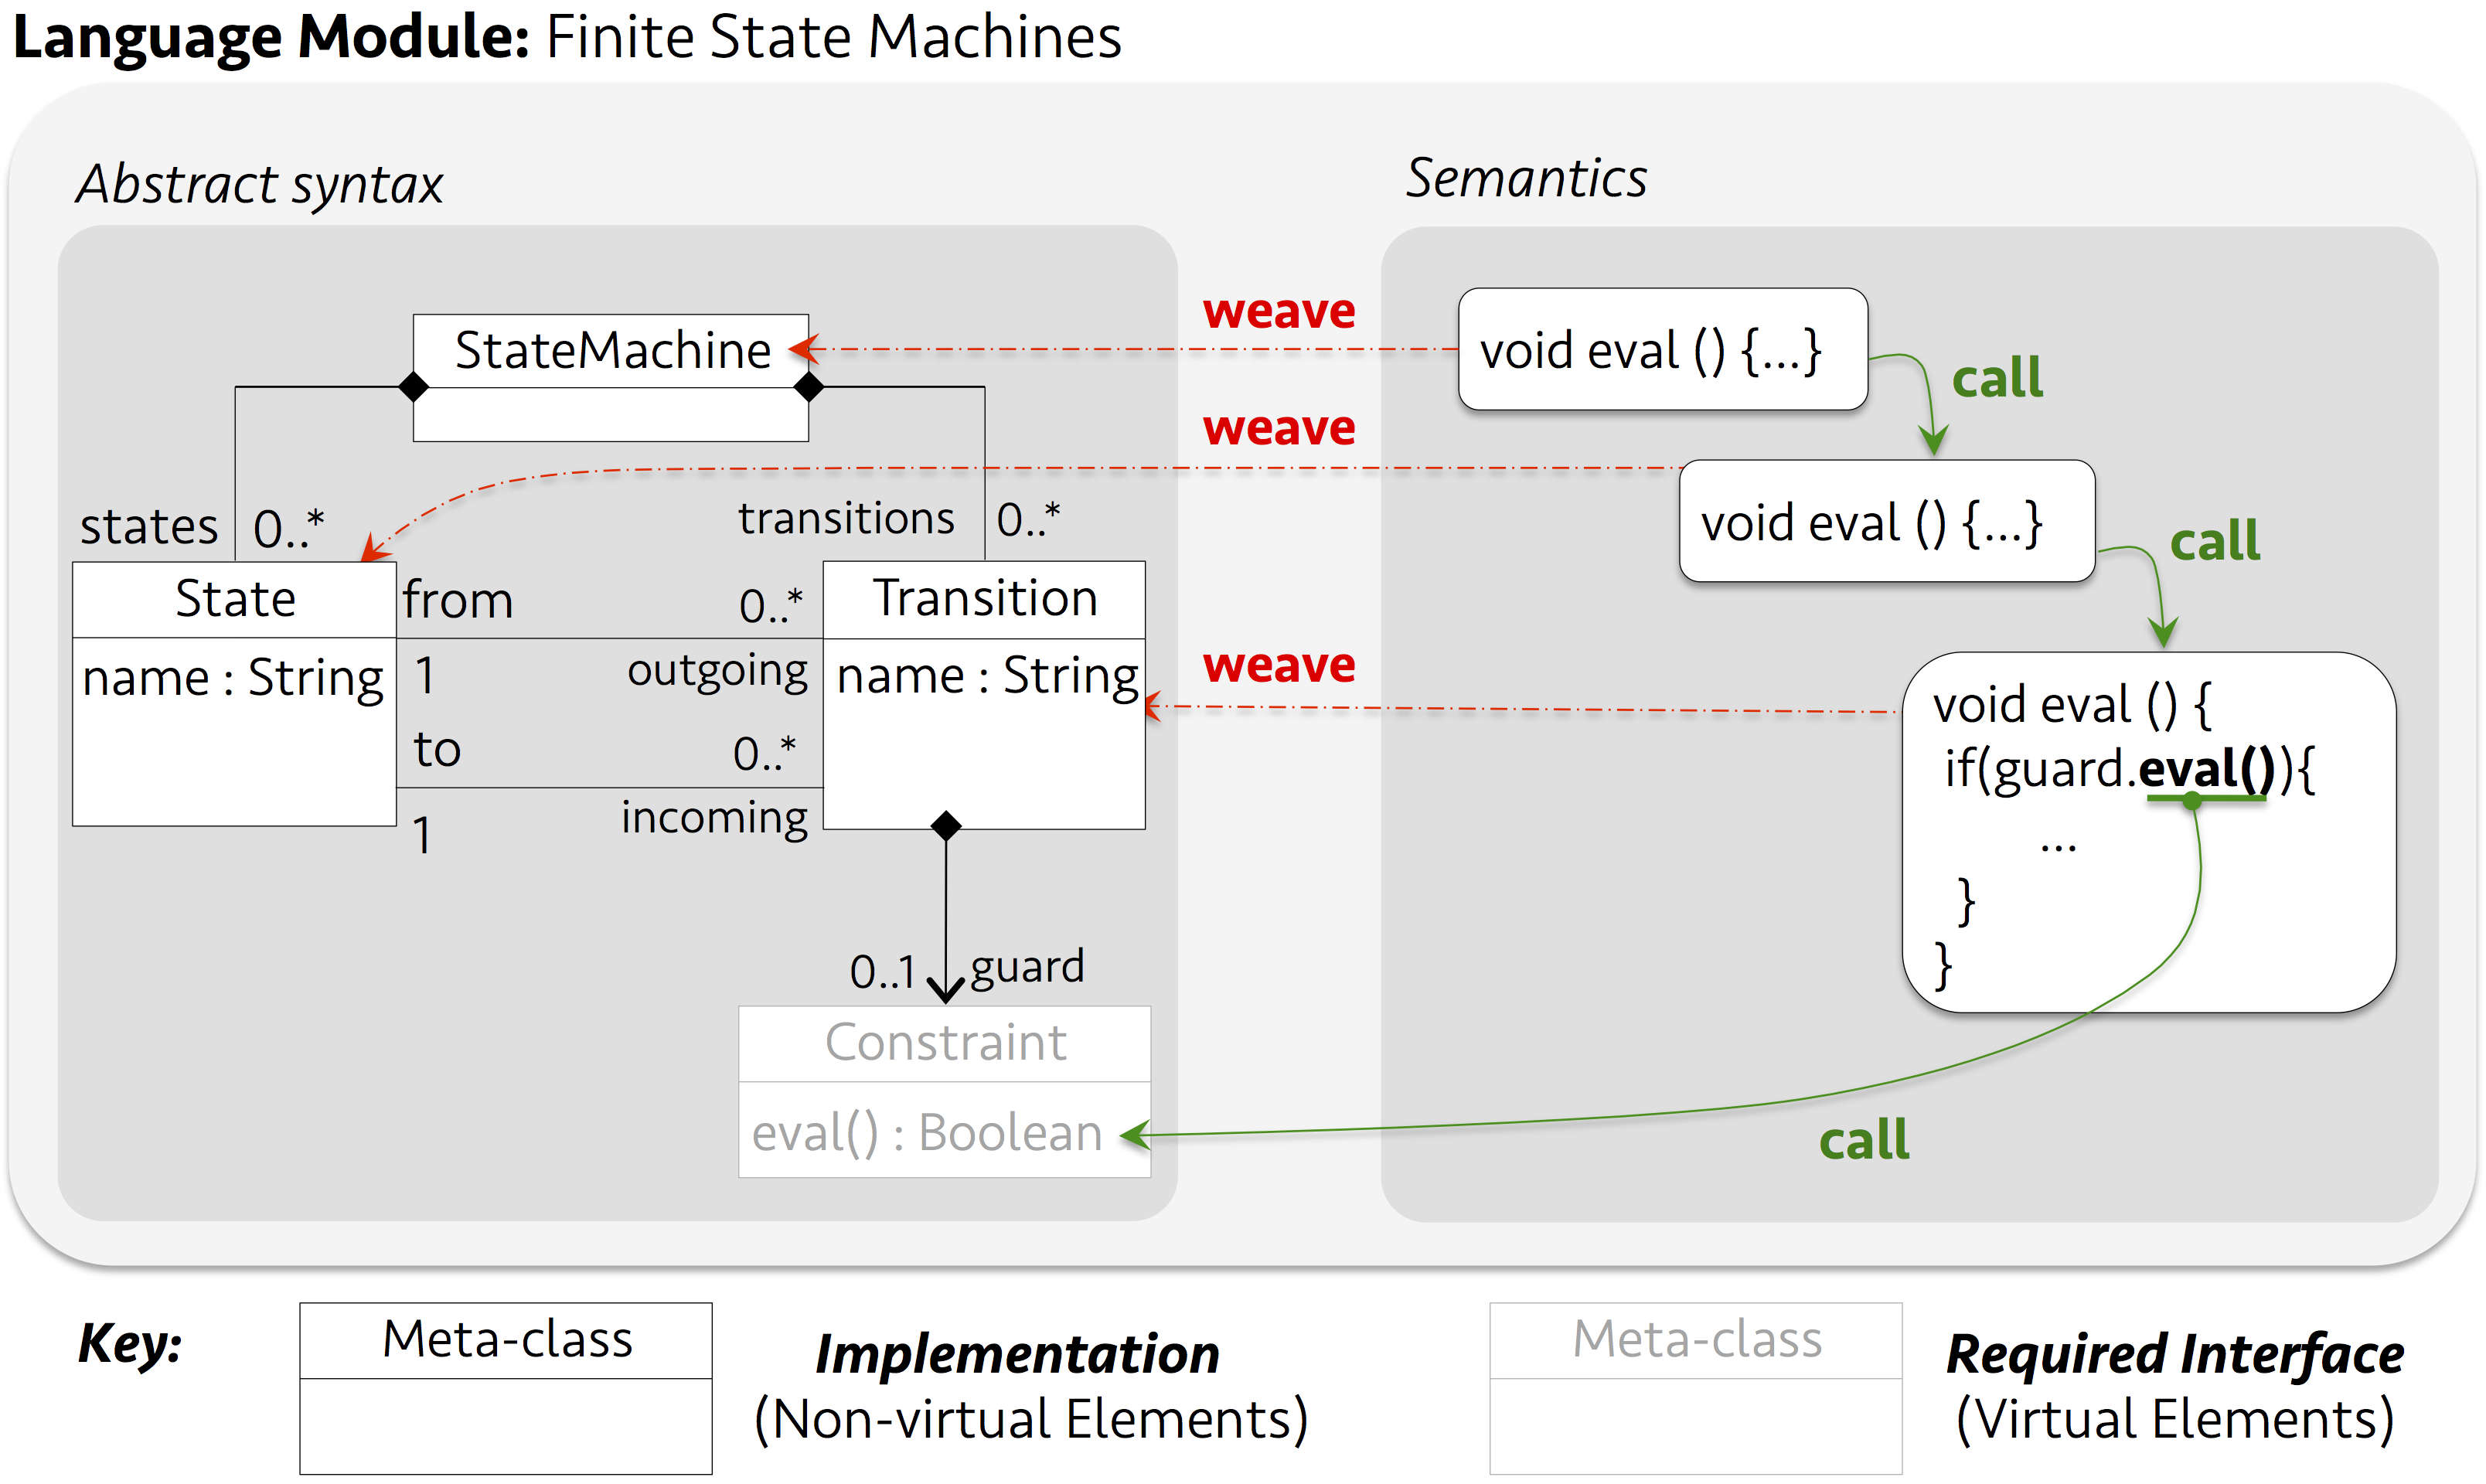
\includegraphics[width=0.86\linewidth]{images/fig-req-example-fig.png}
%  \caption{Example of the use of required interfaces}
%  \label{fig:fig-req-example-fig} 
%\end{figure}

\vspace{2mm}
\textit{\textbf{Provided interfaces.}} The purpose of provided interfaces is to expose the functionality offered by the language module. Consider for example a language module that offers the capability to express and evaluate constraints. Using a providing interface, language designers can express the essential functionality of the module i.e., expression and evaluation of constraints; and hide the implementation details and auxiliary concepts needed to achieve such functionality e.g., context management.

To support the definition of provided interfaces, we propose to extend EMOF with the notion of \textit{module visibility}. This extension allows to classify a certain specification element as either \textsl{\textbf{public}} or \textsl{\textbf{private}} according to its nature. For example, a language designer can classify a meta-class as \textsl{\textbf{public}} meaning that it represents essential functionality of the module so can be used by external modules and it belongs to the provided interface. Naturally, if the meta-class is classified as \textsl{\textbf{private}} it cannot be used by external modules and it cannot be considered as part of the provided interface. Note that the notion of module visibility is different from the notion of visibility already defined in EMOF. The later is associated to  certain access constraints of model elements with respect to the package in which they are implemented.

When encapsulating a language module from a cluster of constructs, all the constructs that are used by external clusters are defined as public.

%Fig. \ref{fig:fig-prov-example-fig} illustrates the use of provided interfaces through the example regarding the constraints module. Since the main functionality of the module is to define and evaluate constraints, the meta-classes included in the provided interface (so those one defined as \textsl{\textbf{public}} in terms of module visibility) are: \textsl{ConstrainedProgram} and \textsl{Constraint} including the operations that implement their semantics.

%\begin{figure}
%  \centering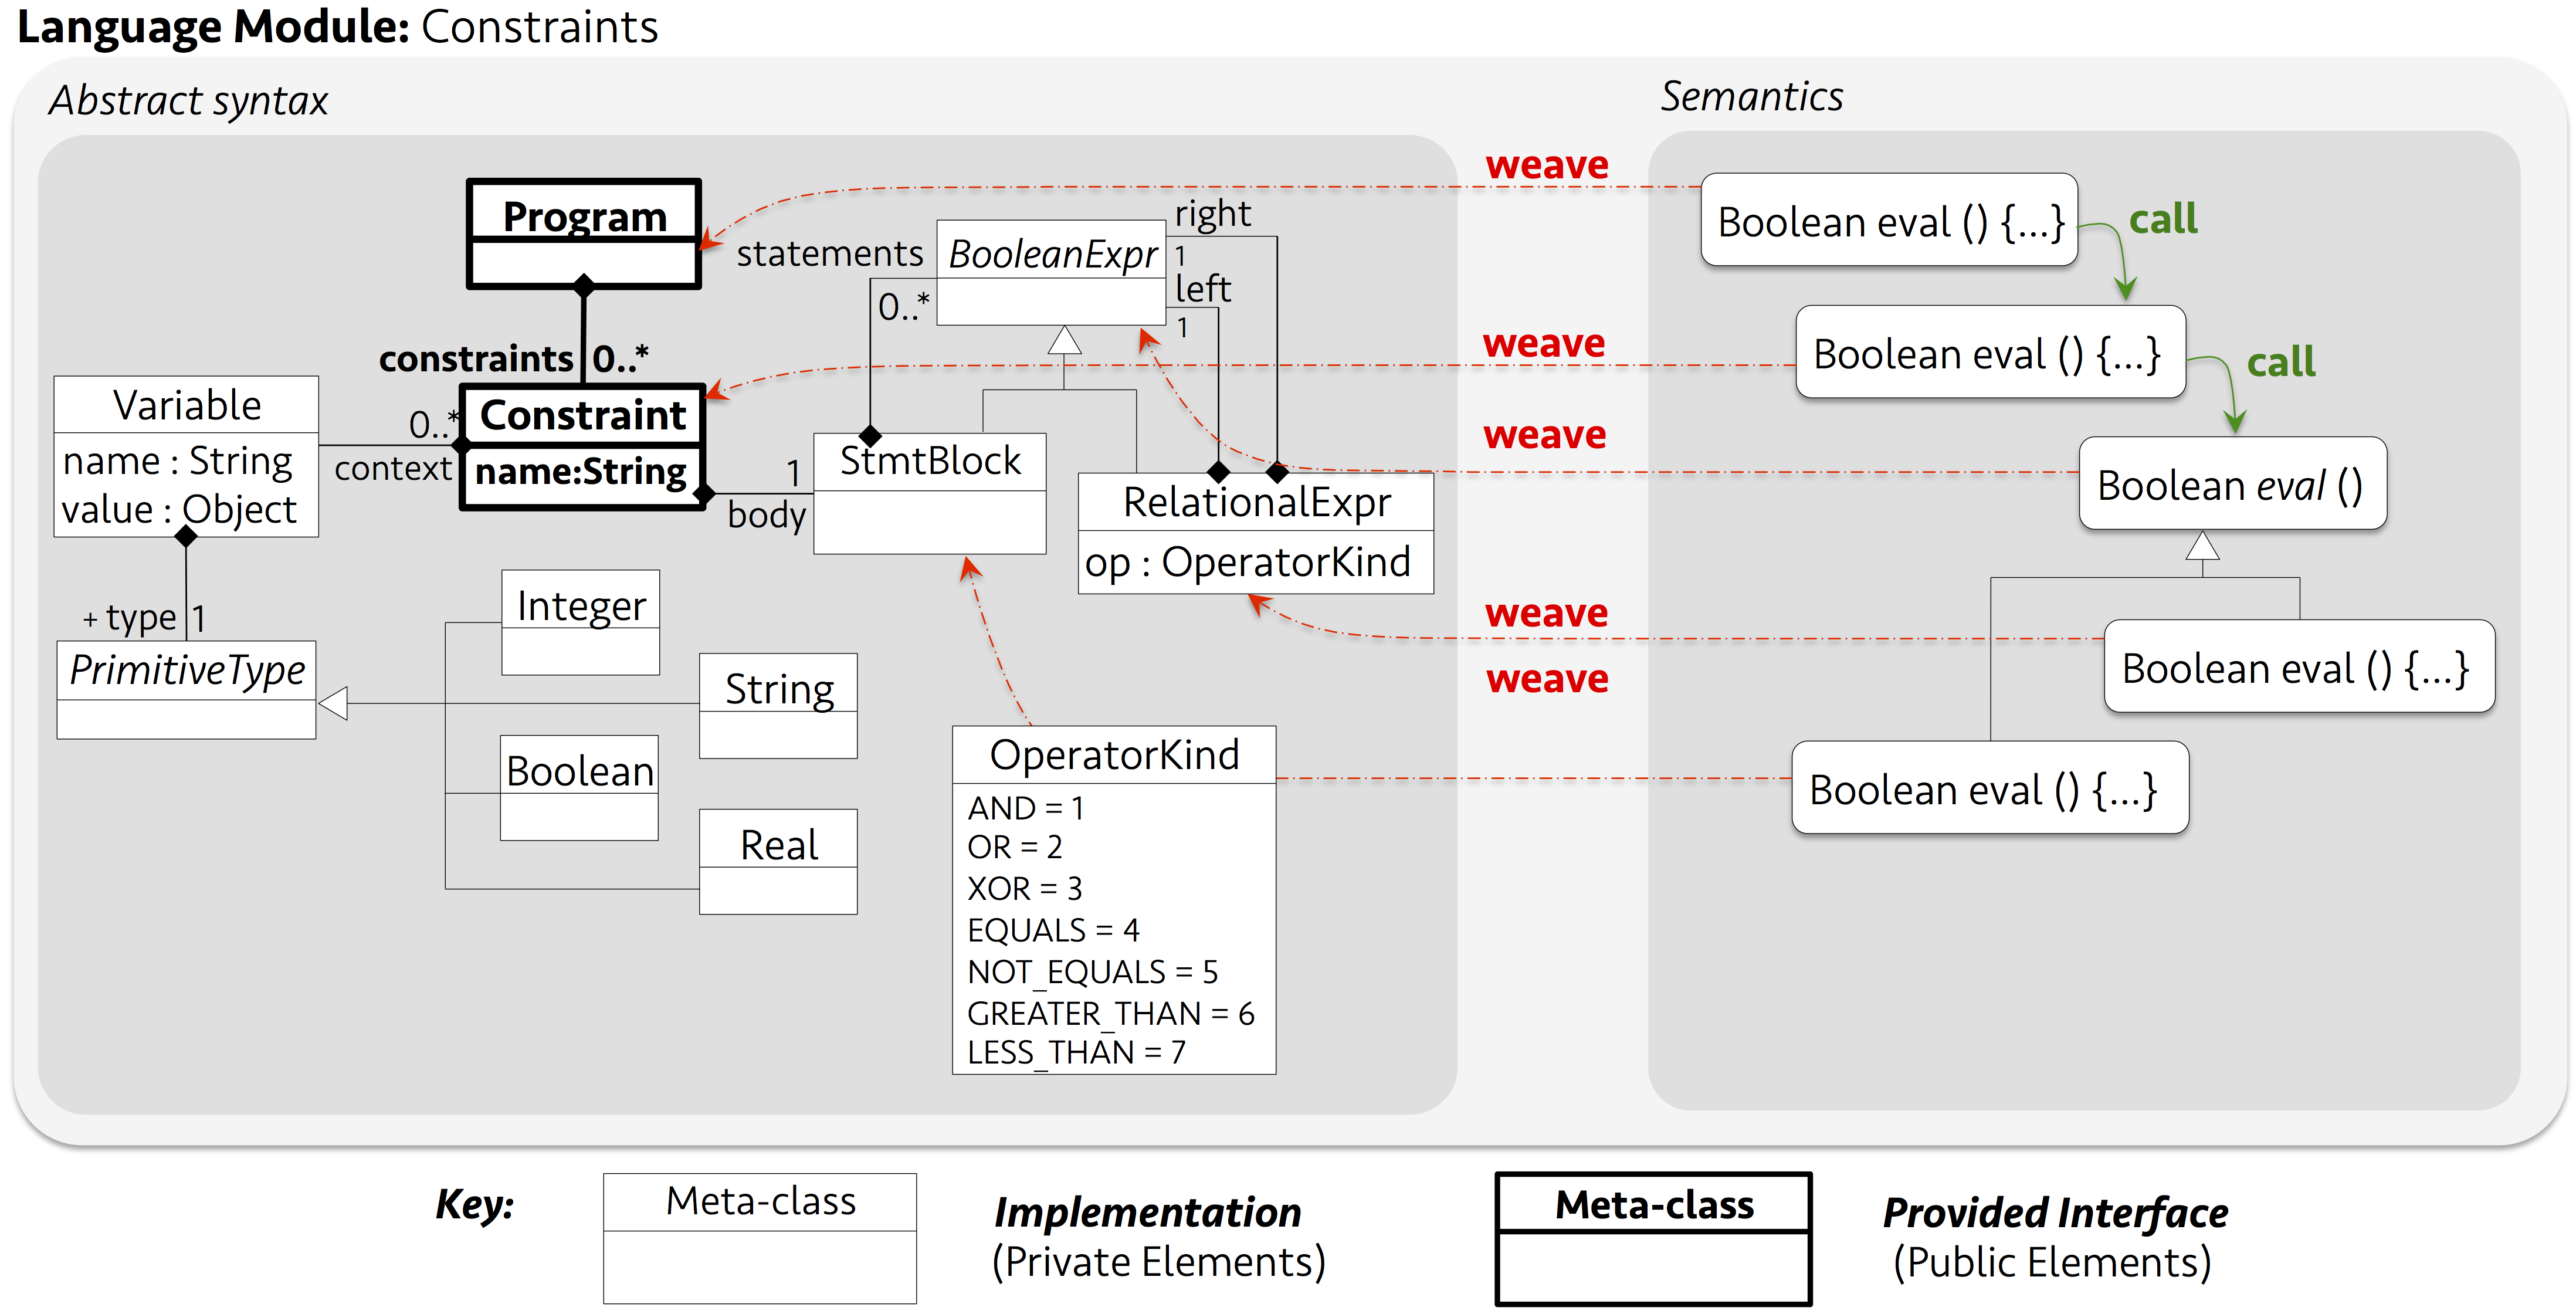
\includegraphics[width=1\linewidth]{images/fig-prov-example-fig.png}
%  \caption{Example of the use of provided interfaces}
%  \label{fig:fig-prov-example-fig}
%\end{figure}

\subsection{Synthesizing Language Variability Models}

Once we have recovered a language modular design for the language product line, we need to represent the existing variability in a model that permits to configure concrete DSLs. To this end, we need to find out an appropriated formalism for express that model, and then to conceive a strategy to synthesize those models from the language modular design. 

\subsubsection{Language Variability. \textbf{How to express it?}}

The challenge towards representing the variability existing in a language product line is that such variability is multi dimensional. Because the specification of a DSL involves several implementation concerns\footnote{Just as traditional general purpose languages, domain specific languages are typically defined through three implementation concerns: abstract syntax, concrete syntax, and semantics \cite{Harel:2004b}.}, then there are several dimensions of variability that we must manage: abstract syntax variability, concrete syntax variability, and semantic variability \cite{Cengarle:2009,Gronniger:2011}.

Abstract syntax variability refers to the capability of selecting the desired language constructs for a particular type of user. Concrete syntax variability refers to the capability of supporting different representations for the same language construct. Finally, semantic variability refers to the capability of supporting different interpretations for the same language construct. As the same as our approach to language modularization, our approach to variability management is scoped to abstract syntax and semantics; concrete syntax --and hence, concrete syntax variability-- is not being considered in the solution. 

%In this section we present a strategy to deal with this type of variability. To this end, we present an approach to represent the variability existing in a language product line. Then, we explain how we can use the variability models to configure concrete DSLs. As the same as our approach to language modularization, our approach to variability management is scoped to abstract syntax and semantics; concrete syntax --and hence, concrete syntax variability-- is not being considered in the solution. 

\vspace{2mm}
\textbf{\textit{Modeling multi-dimensional variability.}} A solution to represent abstract syntax variability and semantic variability should consider two main issues. Firstly, the definition of the semantics has a strong dependency to the definition of the abstract syntax --the domain-specific actions that implement the semantics of a DSL are weaved in the meta-classes defined in the abstract syntax--. Hence, these dimensions of variability are not isolated each other. Rather, the decisions made in the configuration of the abstract syntax variability impact the decisions that can be made in the configuration of the semantic variability. 

The second issue to consider at the moment of dealing with language variability management is that a semantic variation point might be transversal to several meta-classes. Moreover, if the involve meta-classes are introduced by different language modules in the abstract syntax, then the semantic variation point depends of two features. As a result, the relationship between a feature in the abstract syntax and a semantic variation point is not necessarily one-to-one. 

%For example, there is a semantic variation point in hierarchical state machines that corresponds to decide if the state machine follows either the run-to-completion policy or if it supports simultaneous events \cite{Crane:2007}. In any case, the implementation of this semantics involves code in domain-specific actions for the \textsl{StateMachine} and \textsl{Region} meta-classes. 

Currently, we can find several approaches to support multi dimensional variability (e.g., \cite{Rosenmuller:2011}). Some of those approaches have been applied concretely to language product lines \cite{Liebig:2013}. The most common practice is to use feature models to represent all the dimensions of variability. Each dimension is specified in a different tree and dependencies among decisions in those dimensions are expressed as cross-tree constraints. In this article, we propose a different approach based on the combination of feature models with orthogonal variability models. Feature models are used to model abstract syntax variability and orthogonal variability models are used to model semantic variability.

Fig. \ref{fig:languages-variability-modeling} illustrates our approach. At the top of the figure, there is a feature model in which each feature represents a language module. As aforementioned, each language module is composed of a metamodel and a set of domain specific actions. Hence, such a feature model is enough for language product lines where there is not semantic variability i.e., each language module has only one set of domain specific actions. Differently, when there are one or more language modules containing several sets of domain specific actions, then we have semantic variability that must be represented in the variability model. To represent such a variability, we include an orthogonal variability model as illustrated at the bottom of Fig. \ref{fig:languages-variability-modeling} which contains a variation point for each feature that represents a language module with more than one set of domain specific actions.

\begin{figure*}
  \centering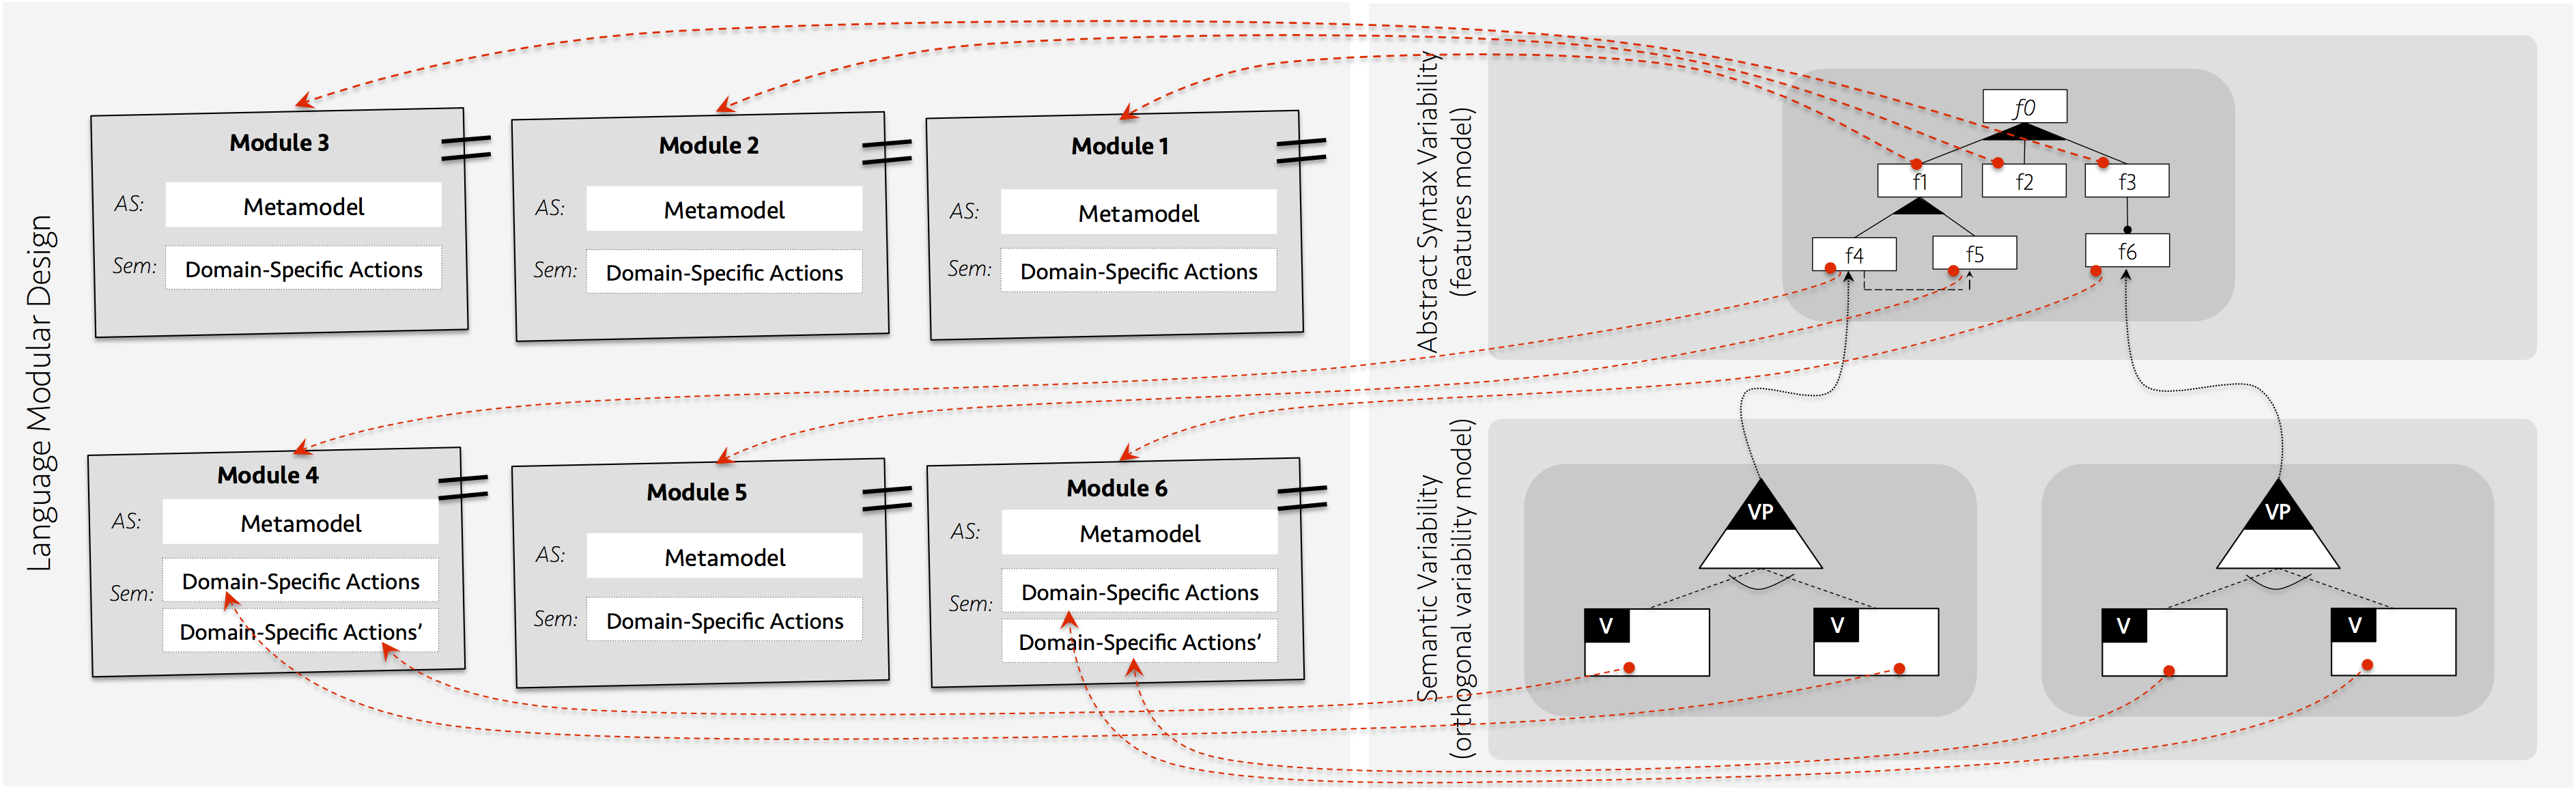
\includegraphics[width=1\linewidth]{images/language-variability-fig.png}
  \caption{Approach to represent multi-dimensional variability in language product lines}
  \label{fig:languages-variability-modeling}
\end{figure*}

\vspace{2mm}
\textit{\textbf{Why orthogonal variability models?}} An inevitable question that we need to answer at this point is: why we use orthogonal variability models instead of using feature models as proposed by current approaches? The answer to this questions is three-fold:

\vspace{2mm}
\textit{(1) The structure of orthogonal variability models is more appropriated.} As explained by Roos-Frantz et al. \cite{Roos-Frantz:2012}, feature models and orthogonal variability models are similar. However, they have some structural differences. One of those differences is that whereas a feature model is a tree that can have many levels, an orthogonal variability model is a set of trees each of which has two levels. Each tree represent one variability point and its children represent variants to that variation point. 

Semantic variation points are decisions with respect to a particular segment of the semantics of a language. Although those decisions can have some dependencies among them, they can hardly be organized in a hierarchy. Indeed, we conducted an experiment where we use feature models to represent semantic variation points, and we always obtained two-level trees: the first level corresponds to the name of the variation point and its children represent the possible decisions. This fact suggests that orthogonal variability models are more appropriated than feature models to represent semantic variability.  

\vspace{2mm}
\textit{(2) The meaning of orthogonal variability models is more appropriated.} According to \cite{Liebig:2013}, a language feature is a characteristic provided by the language which is visible to the final user. This definition can be associated abstract syntax variability and the use of feature models can be appropriated to represented it. All the approaches on language product line engineering use feature models to this end showing that it is possible and appropriated. 

The case of the semantic variability is different. A semantic decision is not a characteristic of a language that we can select or discard. The semantic of a DSL should be always specified if the DSLs is intended to be executable. Rather, a semantic decision is more a variation point that can have different interpretations captured as variants. This vocabulary fits better in the definitions provided by orthogonal variability models. More than features, we have variation points and variants, which also suggest that the use orthogonal variability models is more appropriate to represent semantic variability.

\subsubsection{Language Variability. \textbf{How to synthesize it?}}

Once we established an approach to represent language variability, we define an algorithm to synthesize variability models from a given language modular design. This algorithm produces not only a feature model with the abstract syntax variability, but also an orthogonal variability model representing the semantic variability. An overview of the approach is presented in Fig. \ref{fig:everse-engineering-vm}. 

\begin{figure*}
\centering
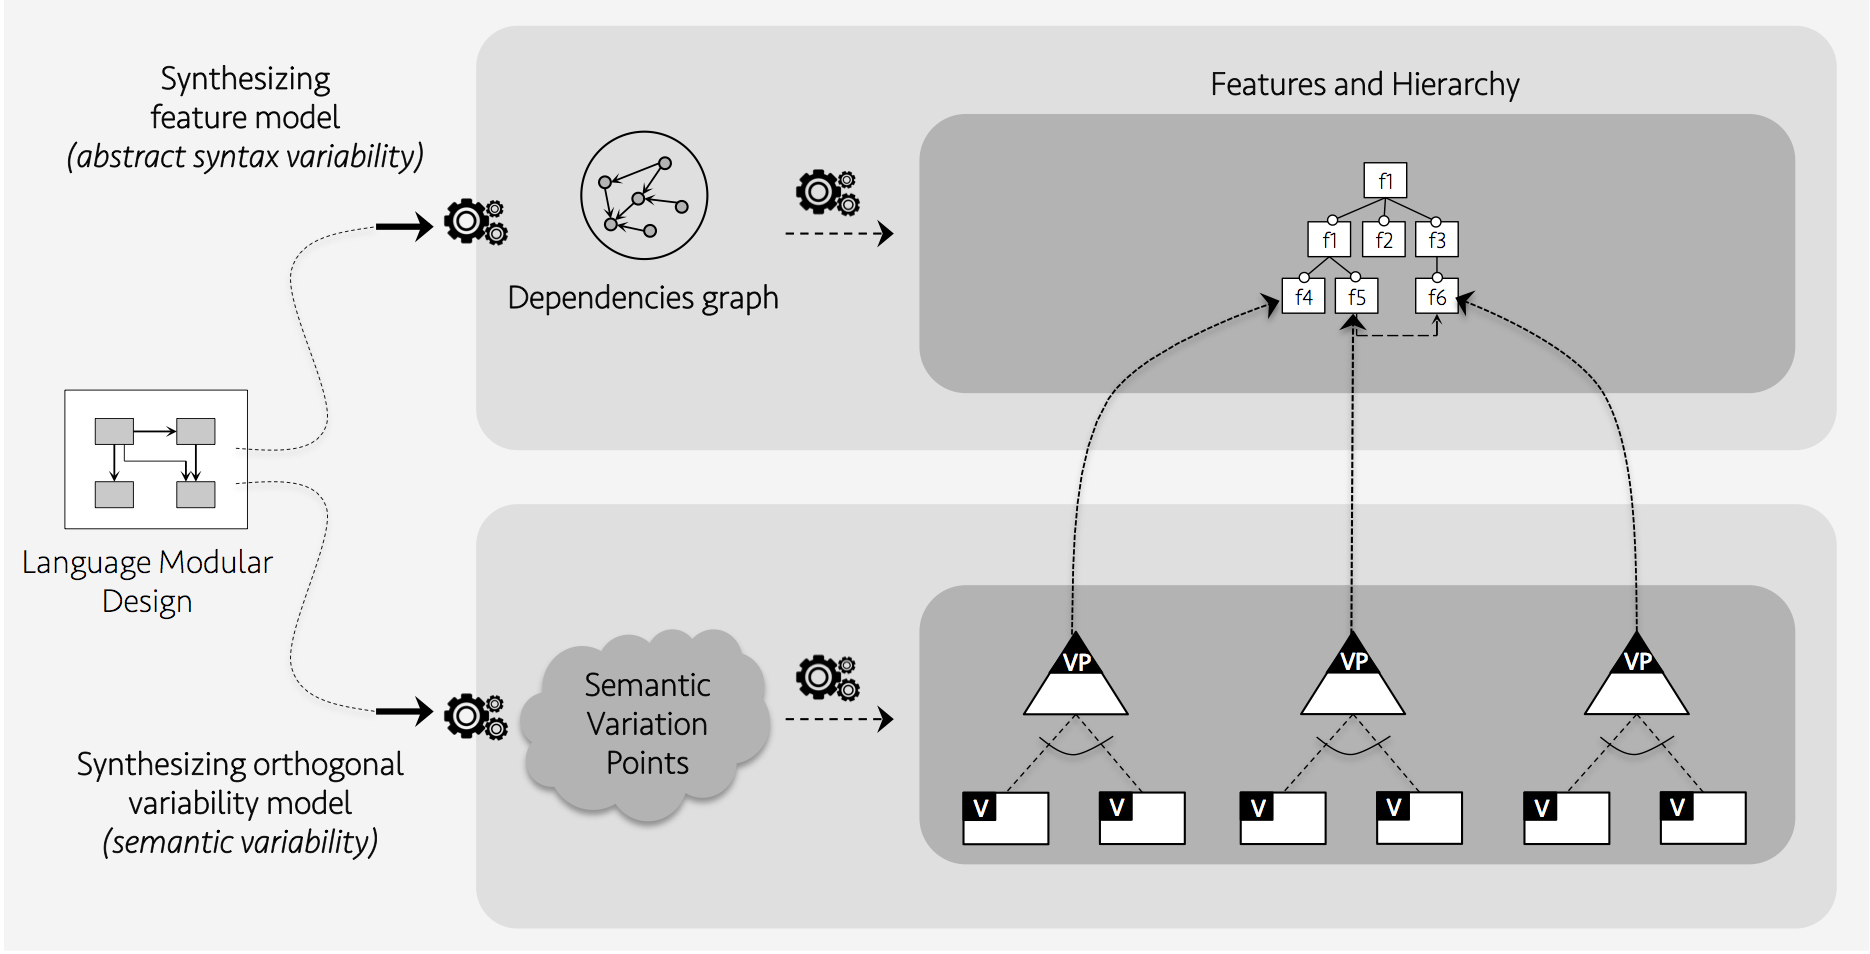
\includegraphics[width=1\linewidth]{images/reverse-engineering-vm.png}
\caption{Reverse-engineering variability models for language product lines}
\label{fig:everse-engineering-vm}
\end{figure*}

\vspace{2mm}
\textit{\textbf{Synthesizing abstract syntax variability.}} The first step to represent the variability of a language product line is to extract the feature model that represents the abstract syntax variability. To this end, we need an algorithm that receives the dependencies graph between the language modules, and produces a feature model which includes a set of features representing the given language modules as well as a set of constraints representing the dependencies among those modules. The produced feature model must guarantee that all the valid configurations (i.e., those that respect the constraints) produce correct DSLs.

In the literature, there are several approaches for reverse engineering feature modules from dependencies graphs (consider for example the approach presented by Assun\c{c}ao et al. \cite{Assuncao:2015}, or the one presented by She et al., \cite{She:2014}). In our case, we opt for an algorithm that produces a simple feature model where each language module is represented in a concrete feature, and where the dependencies between language modules are encoded either by parent-child relationships or by the classical \textit{implies} relationship. Our algorithm was inspired from the approach presented by Vacchi et al. \cite{Vacchi:2013} which fulfills the aforementioned requirements. Besides, it has been applied for the particular case of languages variability. 

The tooling that supports our algorithms is flexible enough to permit the use of other approaches for synthesis of feature model. To this end, we provide an extension point that language designers can use to add new synthesis algorithms. In addition to the one proposed by Vacchi et al. \cite{Vacchi:2013}, we have integrated our approach with the one provided by Assun\c{c}ao et al., \cite{Assuncao:2015}.

%The pseudo-code of the algorithm is introduced below; it is composed of four steps. The first step creates an abstract feature that will be used as the root feature of the variability model. The second step finds the first-level features i.e., the children of the abstract root feature. To this end, it searches all the modules that have not dependencies towards other modules. The third step finishes the hierarchy. It starts by asking the features of the first level to the dependencies they receive. For each of them they create a child. This process is repeated while there are modules that are not included in the model. Finally, we detect these dependencies that are not captured in the hierarchy and we add it in the model in the form of implies relationships. 

\vspace{2mm}
\textit{\textbf{Synthesizing semantic variability.}} Once the feature model encoding abstract syntax variability is produced, we proceed to do the proper with the orthogonal variability model encoding semantic variability. To this end, we need to analyze the results of the process for extracting the language modules. As explained in Section \ref{sec:reverseengineeringmodules}, according to the result of the comparison of the semantics, a language module might have more than one cluster of domain specific actions. This occurs when the two DSLs share constructs that are equal in terms of the abstract syntax, but differ in their semantics. Since this is the definition of semantic variation point, we materialize those clusters in semantic variation points of an orthogonal variability model.

To do this, we scan all the language modules. For each one, we verify if it has more than one cluster of domain specific actions. If so, we create a semantic variation point where each variation references one cluster. Finally, the semantic variation point is associated with the feature that represents the language module owning the clusters. 

\subsubsection{DSL Variants Configuration}

There are two issues to consider to support configuration of DSL variants in language product line engineering. First, the multi-dimensional nature of the variability in language product lines, supposes the existence of a configuration process supporting dependencies between the decisions of different dimensions of variability. For example, decisions in the abstract syntax variability may impact decisions in semantic variability. Second, language product lines often require multi-staged languages configuration. That is, the possibility of configuring a language in several stages and by different stakeholders.

Multi-staged configuration was introduced by Czarnecki et al. \cite{Czarnecki:2004} for the general case of software product lines, and discussed by Dinkelaker et al. \cite{Dinkelaker:2010} for the particular case of DSLs. The main motivation to support such functionality is to transfer certain configuration decisions to the final user so he/she can adapt the language to exactly fits his/her needs \cite{Dinkelaker:2010}. In that case, the configuration process is as follows: the language designer provides an initial configuration. Then, the configuration is continued by the final user that can use the DSL as long as the configuration is complete. In doing so, it is important to decide what decisions correspond to each stakeholder.

Suppose the scenario introduced in Fig. \ref{fig:languages-configuration-modeling} where the language designer is responsible to configure the abstract syntax variability whereas the language user is responsible to configure the semantics. When the language designer finishes its configuration process, the orthogonal variability models will be available so the final user can perform the configuration of the semantics. This orthogonal variability model will only include the variation points that are relevant to the features included in the configuration of the abstract syntax. Moreover, because each of the semantic variation points are represented separately in a different tree, then we can imagine a scenario where the language designer is able to configure not only the abstract syntax but also some semantic variation points, and then delegate to the final user only the decisions that he/she can take according to its knowledge. 

\begin{figure}
  \centering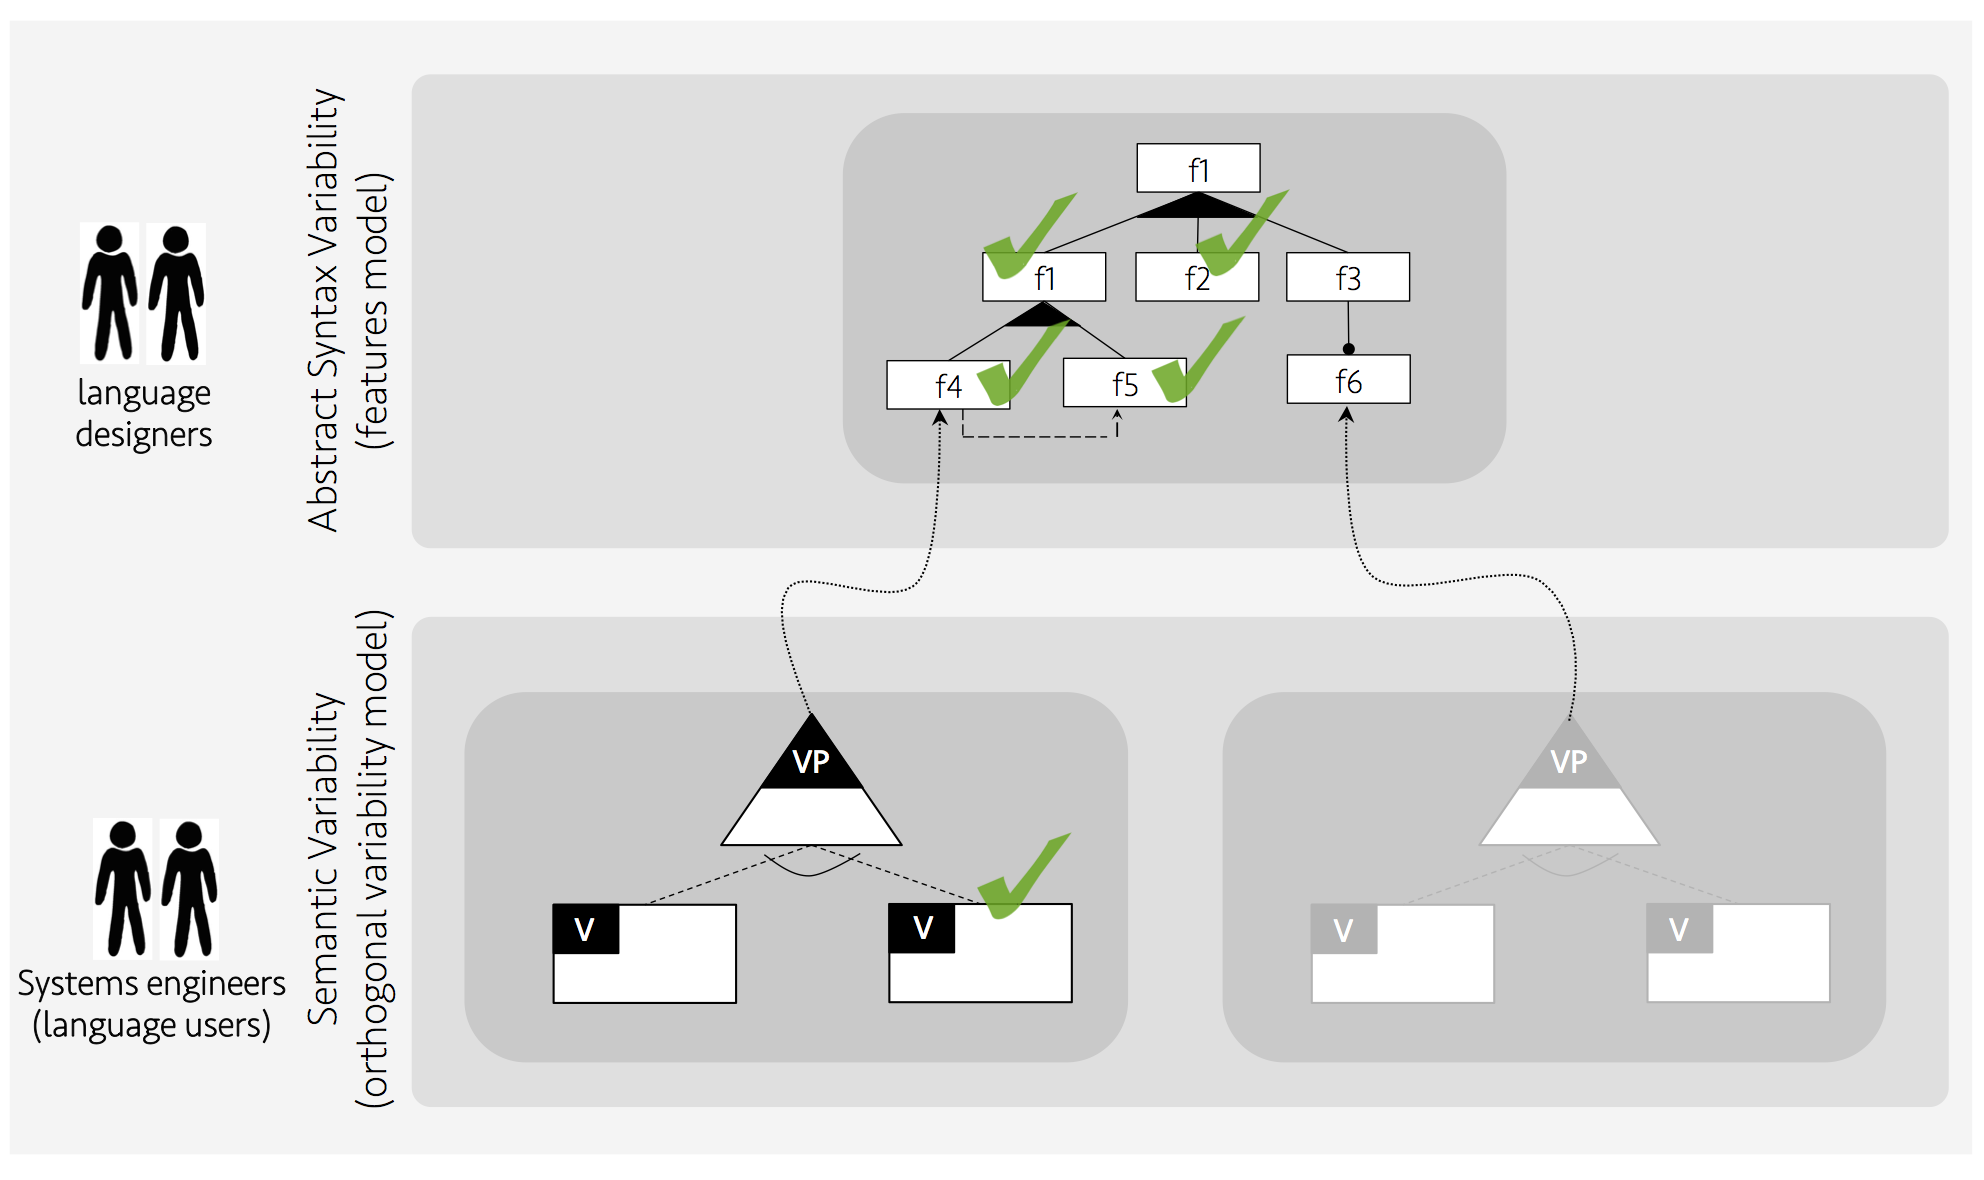
\includegraphics[width=1\linewidth]{images/languages-configuration-fig.png}
  \caption{Approach to support multi-staged configuration of language product lines}
  \label{fig:languages-configuration-modeling}
\end{figure}

\subsection{Language Modules Composition}

The final step of the language product line engineering process is the composition of the language modules corresponding to the configuration indicated in the variability models. This composition process starts by checking the compatibility between the required and provided interfaces of the involved modules. Then, the specification of the modules are merged to produce a complete DSL variant.  

\vspace{2mm}
\textbf{\textit{Compatibility checking.}} To establish a compatibility checking mechanism between provided and required interfaces, we need to conciliate two different (and potentially conflicting) issues. Firstly, such a compatibility checking must guarantee safe composition of the involved language modules. Hence, we need to verify that the functionality offered by the provided interface actually fulfills the needs of required interface. Secondly, there must be some place for substitutability. Hence, compatibility checking should offer certain flexibility that permits to perform composition despite some differences in their definitions. This is important because when language modules are development independently of each other, their interfaces and implementations not always match \cite{Gschwind:2012}.

To deal with the aforementioned issues, we propose an approach for compatibility checking which is at the same time strict enough to guarantee safe composition, and flexible enough to permit substitutability under certain conditions. We extract both required and provided interfaces in the form of \textit{model types} \cite{Steel:2007}. The model type corresponding to the required interface contains the required specification elements of a language module whereas the model type corresponding to the provided interface the model type contains its public specification elements \footnote{The relationship between a model type and a language module is called \textsl{\textbf{implements}} and it is introduced by Degueule et al. \cite{Degueule:2015a}.}. Then, we perform compatibility checking by checking the sub-typing relationship --introduced by Guy et al. \cite{Guy:2012}-- between the model types corresponding to the provided and the required interfaces. This relationship imposes certain constraints that guarantee safe composition while permitting some freedom degrees thus introducing some flexibility. %In particular, under this definition of sub-typing the most obvious manner to guarantee safe composition is to check two conditions: (1) all the needs expressed in the requiring model type are furnished in the providing model type (\textbf{total} sub-typing); and (2) the two model types have exactly the same shape (\textbf{isomorphic} sub-typing). However, this definition of sub-typing also provides two dimensions of flexibility: \textbf{partial} sub-typing and \textbf{non-isomorphic} sub-typing. 

%The main principle behind partial sub-typing is that not all the needs expressed in the required model type must be provided by the provided one. In that case, compatibility checking corresponds to verify that the sub-set of elements that match in the model types are compatible. Then, the result of the composition is a third language module with a resulting required interface that contains those needs that have not been satisfied by the providing language module. 

%As an example suppose a language module for finite state machines that needs not only constraints for expressing guards in the transitions, but also action scripting constructs to express the behavior of the states. In such a case, a constraint module will fulfill the first need but not the second one. Thanks to partial sub-typing, we can perform compatibility checking only on the constructs associated to the constraints and, if they are compatible, then compose those language modules. The result will be a language module having the constructs for state machines and constraints but that still needs action scripting constructs defined in its required interface.

%The principle behind isomorphic sub-typing is that the needs in the requiring interface are not always expressed exactly as the functionality offered by the providing module is expressed in the providing interface. For example, model type in Fig. \ref{fig:fig-req-example-fig} expresses the needs in terms of constraints of state machines through a class \textsl{Constraint} with an operation \textsl{eval()}. If we want to use OCL to satisfy these needs, then we will find that there is not a class constraint but \textsl{OclExpr}. Besides, the operational semantics might be implemented differently. In this case, we need an adapter that permit to find the correspondences among the elements of the model types. 

\vspace{2mm}
\textit{\textbf{Merging modules' specifications.}} The process of merging the specification of a set of language modules is performed in two phases. First, there is a matching process that identifies one-to-one matches between required and public elements from the required and provided interface respectively. This match can be identified automatically by comparing names and types of the elements (where applicable). However, the match can be also specified manually in the case of non-isomorphism.

Once the match is correctly established, the composition process continues with a merging algorithm that replaces virtual elements with public ones. When the process is finished, we re-calculate both provided and required interfaces. The provided interface of the composition is re-calculated as the sum of the public elements of the two modules under composition. In turn, the required interface of the composition is re-calculated as the difference of the required interface of the required module minus the provided interface of the providing module. 

